\section{Digitale Regelung}

\subsection{Regelkreis mit digitalem Regler}{214}

Ein Regelkreis mit digitalem Regler hat folgende Struktur:

\smallskip

\begin{minipage}[t]{0.64\columnwidth}
    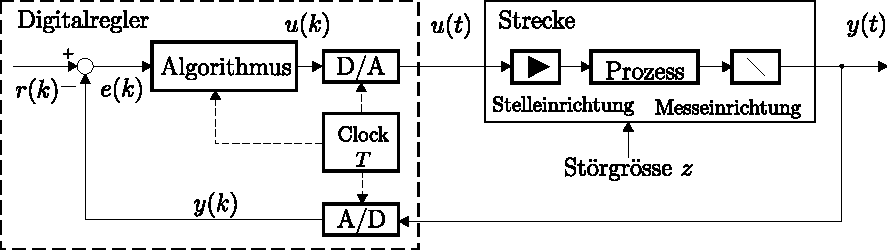
\includegraphics[width=\columnwidth, align=t]{images/dig_reg_regelkreis.pdf}
\end{minipage}
\hfill
\begin{minipage}[t]{0.34\columnwidth}
    \begin{outline}
        \1 Strecke ändert \textbf{nicht}
        \1 Regler arbeitet \textbf{zeitdiskret}
        \1 Zentraler Clock
            \2 Abtastzeit $T$
        \1 Schnittstellen:\\
            A/D bzw. D/A Wandler
    \end{outline}
\end{minipage}


\subsubsection{Vorteile / Nachteile digitale Regler}{215-217}

\begin{itemize}
    \item[+] Struktur / Parameter des Reglers einfach veränderbar \textrightarrow\ adaptive Regelung
    \item[+] Entwicklungsumgebungen (z.B. Simulink) erlauben Simulation des Reglers und anschliessende Code-Generierung
    \item[+] Nichtlineare Regleralgorithmen sind einfach implementierbar 
    \item[+] Digitale Regler können Teil eines hierarchischen Regelsystems sein
    \item[+] Einfacher, schneller Wechsel zwischen verschiedenen Reglern möglich
    \item[+] (Intelligente) Sensoren liefern Daten digital, nicht analog
    \item[-] Wertquantisierung der Signale \textrightarrow\ Quantisierungsrauschen
    \item[-] Zeitquantisierung \textrightarrow\ Totzeit von ca. $50\, \%$ der Abtastzeit $T$ 
    \item[-] Rundungsfehler aufgrund von rechnerischer Zahlendarstellung   
\end{itemize}
%-----------------------------------------------------------------------------------------------------------------------------------
\subsubsection{Diskretisierung eines Integrators}

Kontinuierlich:

\[
G(s)=\frac1s
\]

Rechteck vorwärts:

\[
G(z)=\frac{T}{z-1}
\]

Rechteck rückwärts:

\[
G(z)=\frac{Tz}{z-1}
\]

Trapezregel (Tustin):

\[
G(z)=
\frac{T}{2}
\frac{z+1}{z-1}
\]

\para{Stabilität}

Kontinuierlich:

\[
\Re(\lambda)<0
\]

Diskret:

\[
|z_i|<1
\]

(Pole innerhalb Einheitskreis)
%-----------------------------------------------------------------------------------------------------------------------------------

\subsection{Signale im digitalen Regelkreis}{184}
\label{Signale im digitalen Regelkreis}

Die im Digitalregler verarbeiteten Signale $y(k)$, $r(k)$, $e(k)$ und $u(k)$ sind keine Funktionen der Zeit, sondern \textbf{Folgen von Werten}!

\begin{outline}
    \1 Sensorseitig wird jeweilt zum Zeitpunkt $t = k \cdot T$ das Signal $y(t)$ abgetastet
        \2 \textbf{TP:} Analoges Tiefpassfilter \textrightarrow\ Anti-Aliasing
    \1 Aktorseitig wird mit einem \textbf{ZOH}-Halteglied (Zero-Order-Hold) aus dem diskreten Signal $u(k)$ das Signal $u(t)$ erzeugt, welches während eines Abtastintervalls konstant ist
\end{outline}

\vspace{-0.2cm}

\begin{center}
    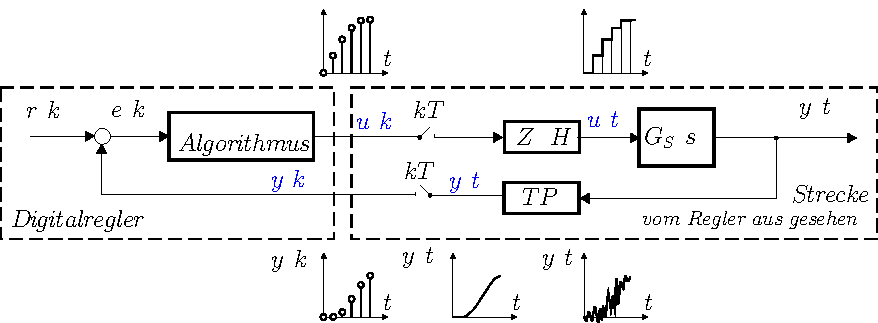
\includegraphics[width=0.9\columnwidth]{images/dig_reg_regelkreis_signale.pdf}
\end{center}

\vspace{-0.2cm}

Damit das Zusammenspiel zwischen digitalem Regler und analoger Strecke korrekt funktioniert, muss die Schnittstelle 'gut funktionieren'.
Da diese Schnittstelle aus A/D- bzw. D/A-Wandlern besteht, müssen die Effekte rund um die \textbf{Signal-Quantisierung} betrachtet werden.


\subsubsection{Quantisierung der Signalwerte / Sättigung}{219-220}

Quantisierung und Sättigung sind \textbf{nichtlineare Effekte}. Es ist daher wichtig, die Auflösung der A/D- und D/A-Wandler geeignet zu wählen.

\smallskip

\begin{outline}
    \1 Zu grobe Quantisierung der Signalwerte führt zu \textbf{Nichtliearität}
    \1 Zu feine Quantisierung der Signalwete hat \textbf{keinen negativen Einfluss} auf Regler
        \2 Ist jedoch teuer
\end{outline}


\subsubsection{Wahl der Abtastzeit $\bm{T}$}{220-221}

Im Prinzip gilt: \textbf{Je kleiner die Abtastzeit $\bm{T}$ eines Reglers ist, desto besser kann der Regler arbeiten}.

\smallskip

\begin{outline}
    \1 Wird die Abtastzeit zu klein gewählt, können numerische Probleme entstehen
    \1 Wird die Abtastzeit zu gross gewählt, kommt es zu Überschwingen oder bis zur Destabilisierung des Systems
\end{outline}

\smallskip

Damit die Abtastzeit $T$ des Reglers entsprechend gewählt werden kann, gibt es 'Faustregeln', bei welchen die Führungsgrösse, der offene Regelkreis 
(Regelstrecke) oder der geschlossene Regelkreis betrachtet wird.

\medskip

\paragraph{Faustregel: Abtastzeit mittels Führungsgrösse}

Das Spektrum der Führungsgrösse $r(t)$ ist begrenzt durch $\omega_r$. Damit bei der Abtastung von $y(t)$ keine Informationen verloren gehen,
wird das Nyquist-Theorem meist um \cbl{Faktor 10} übererfüllt.

\vspace{-0.2cm}

$$ \omega_s = \frac{2 \pi}{T} \leq \cbl{10} \cdot 2 \, \omega_r $$


\columnbreak


\paragraph{Faustregel: Abtastzeit mittels Regelstrecke}

\begin{minipage}[c]{0.45\columnwidth}
    Aus der \textbf{Schrittantwort der Regelstrecke} werden mittels \textbf{Wendetangente} die folgenden Parameter herausgelesen und damit die Abtastzeit bestimmt. 

    \smallskip

    \textrightarrow\ Wenn sich die verschiedenen \textbf{Empfehlungen widersprechen}, ist tendenziell der \textbf{kleinere Wert} als Abtastzeit $T$ zu wählen!
\end{minipage}
\hfill
\begin{minipage}[c]{0.53\columnwidth}   
    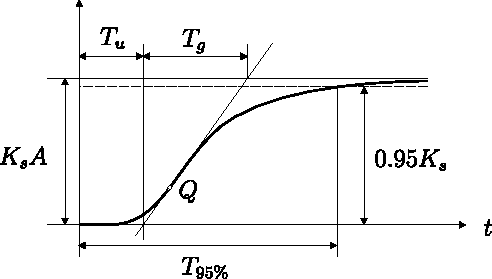
\includegraphics[width=\columnwidth, align=t]{images/dig_reg_schrittantwort_wendetangente.pdf}
\end{minipage}

\vspace{-0.1cm}

\begin{ctabular}{lll}
    \toprule
    \textbf{Kennwert}   & \textbf{Abtastzeit}                                   & \textbf{Kommentar}                \\
    \midrule
    $T_u$               & $0.1 \cdot T_u \leq T \leq 0.25 \cdot T_u$            & Prozess mit ausgeprägter Totzeit  \\
    \midrule
    $T_g$               & $T \leq 0.1 \cdot T_g$                                & $T_g \gg T_u$                     \\
    \midrule
    $T_{95\%}$          & $0.05 \cdot T_{95\%} \leq T \leq 0.1 \cdot T_{95\%}$  &                                   \\
    \bottomrule
\end{ctabular}

\smallskip


\paragraph{Faustregel: Abtastzeit mittels geschlossenem Regelkreis}

\textbf{Voraussetzung:} Es existiert bereits ein Regler in Analogtechnik oder in der Simulation.

\smallskip

\begin{minipage}[t]{0.45\columnwidth}
    Aus der \textbf{Schrittantwort des geschlossenen Regelkreises} werden die folgenden Parameter herausgelesen und damit die Abtastzeit bestimmt.

    \smallskip

    \textrightarrow\ Wenn sich die verschiedenen \textbf{Empfehlungen widersprechen}, ist tendenziell der \textbf{kleinere Wert} als Abtastzeit $T$ zu wählen!
\end{minipage}
\hfill
\begin{minipage}[t]{0.53\columnwidth}   
    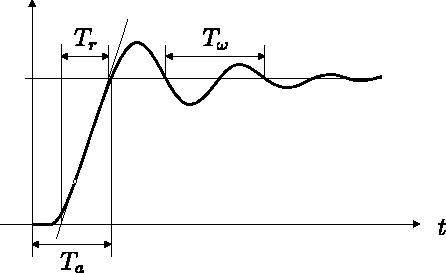
\includegraphics[width=\columnwidth, align=t]{images/dig_reg_schrittantwort_kennwerte.pdf}
\end{minipage}

\vspace{-0.1cm}

\begin{ctabular}{ll}
    \toprule
    \textbf{Kennwert}   & \textbf{Abtastzeit}                           \\
    \midrule
    $T_a$               & $0.05 \cdot T_a \leq T \leq 0.1 \cdot T_a$    \\
    \midrule
    $T_r$               & $0.05 \cdot T_r \leq T \leq 0.1 \cdot T_r$    \\
    \midrule
    $T_{\omega}$        & $T \leq 0.05 \cdot T_{\omega}$                \\
    \bottomrule
\end{ctabular}



\subsubsection{Anti-Aliasing Filter}{222-223}

Ein Signal $y(t)$ wird periodisch mit Abtastzeit $T$, bzw. mit Abtastfrequenz $\omega_s$ abgetastet. 
Die Folge der abgetasteten Werte ist dann $y(k)$.

\vspace{-0.5cm}

$$ y(t) = A \cdot \cos(\omega_0 t) \quad \underrightarrow{\text{sampling: } \omega_s} \quad y(kT) = A \cdot \cos(\omega_0 \cdot kT) \qquad \text{mit } \omega_s = 2 \pi f_s = \frac{2 \pi}{T} $$

\vspace{-0.2cm}

Dieselbe Folge resultiert aber auch, wenn ein Signal $\tilde{y}(t) = A \cdot \cos\left([n \cdot \omega_s \pm \omega_0] \cdot t \right)$ mit $\omega_s$ abgetastet wird ($n$ ganzzahlig). \\
Hat solch ein Signal $\tilde{y}(t)$ Frequenzanteile, die \textbf{oberhalb der Nyquistfrequenz $\bm{\omega_N}$} liegen, so werden diese
Anteile ebenfalls ins Frequenzband $\omega = [0, \, \omega_N]$ abgebildet. 

\smallskip

Frequenzanteile, welche oberhalb der Nyquistfrequenz $\omega_N$ liegen, müssen deshalb mit einem \textbf{Anti-Aliasing-Filter (Tiefpass)} herausgefiltert werden.
Somit ist das Nyquist-Kriterium erfüllt.

\vspace{-0.2cm}

$$ \omega_N = \frac{\omega_s}{2} = \frac{\pi}{T} \quad \Leftrightarrow\ \quad \omega_s > 2 \cdot \omega_{\rm Signal} $$


\subsection{Reglerentwurf -- direkt vs. indirekt}{224-225}

\begin{minipage}[t]{0.48\columnwidth}
    \raggedright
    \begin{outline}
        \1  Indirekter digitaler Reglerentwurf
            \2 $G_S(s)$ \textrightarrow\ 'links herum' \textrightarrow\ $G_{R,I}(z)$
            \2 Zeitkontinuerlicher Regler wird zeitdiskret approximiert
    \end{outline}
\end{minipage}
\hfill
\begin{minipage}[t]{0.48\columnwidth}
    \raggedright
    \begin{outline}
        \1 Direkter digitaler Reglerentwurf
            \2 $G_S(s)$ \textrightarrow\ 'rechts herum' \textrightarrow\ $G_{R,D}(z)$
            \2 'Digitale Natur' des Reglers von Anfang an berücksichtigt
    \end{outline}
\end{minipage}


\begin{center}
    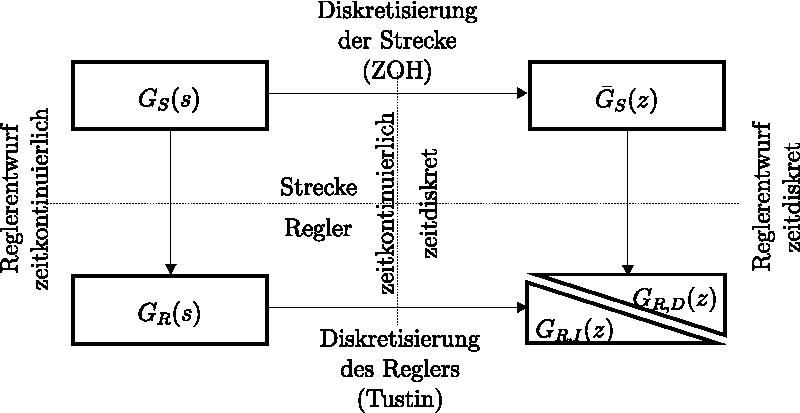
\includegraphics[width=0.8\columnwidth, align=t]{images/dig_reg_reglerentwurf.pdf}
\end{center}

% \begin{minipage}[t]{0.51\columnwidth}
%     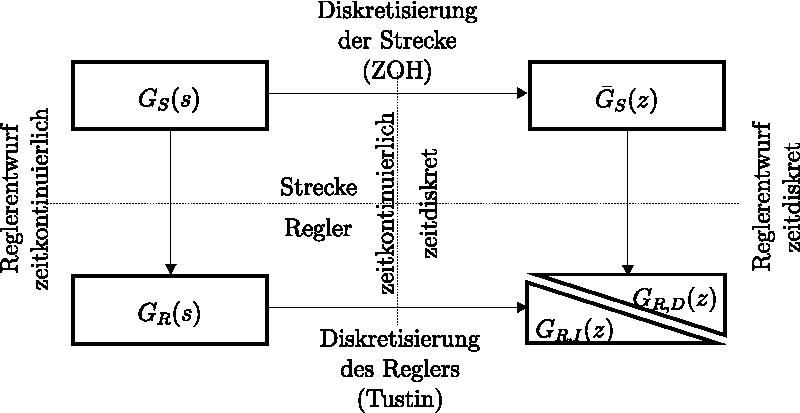
\includegraphics[width=\columnwidth, align=t]{images/dig_reg_reglerentwurf.pdf}
% \end{minipage}
% \hfill
% \begin{minipage}[t]{0.48\columnwidth}
%     \raggedright
%     \begin{outline}
%         \1  \textbf{Indirekter digitaler Reglerentwurf}
%             \2 $G_S(s)$ \textrightarrow\ 'links herum' \textrightarrow\ $G_{R,I}(z)$
%             \2 Zeitkontinuerlicher Regler wird zeitdiskret approximiert
%         \1 Direkter digitaler Reglerentwurf
%             \2 $G_S(s)$ \textrightarrow\ 'rechts herum' \textrightarrow\ $G_{R,D}(z)$
%             \2 'Digitale Natur' des Reglers von Anfang an berücksichtigt
%     \end{outline}
% \end{minipage}

